\chapter{Introduction}
\label{chp1}
\section{Introduction}
Now a day�s education plays a great role in development of any country. Many of education organizations try to increase education quality. One of the aspects of this improvement is managing of school resources. School Management System carried on by any individual or institution engaged in providing a services to students, teachers, guardians and other persons are intermediary that performs one or more of the following functionalities � Student Admission, Employee Registration, Student List, Employee List, Student Attendance, Employee Attendance, Student Routine, Result Management, Payroll \& Accounts. School Management System (SMS) is such a service which provides all services for an educational institute to make your life easier and faster by assuring its performance. Easy User Management System, Easy Admission Process, Easy Attendance System\cite{burke2003practice}.
\begin{figure}[H]  %h=positioning
\begin{center}
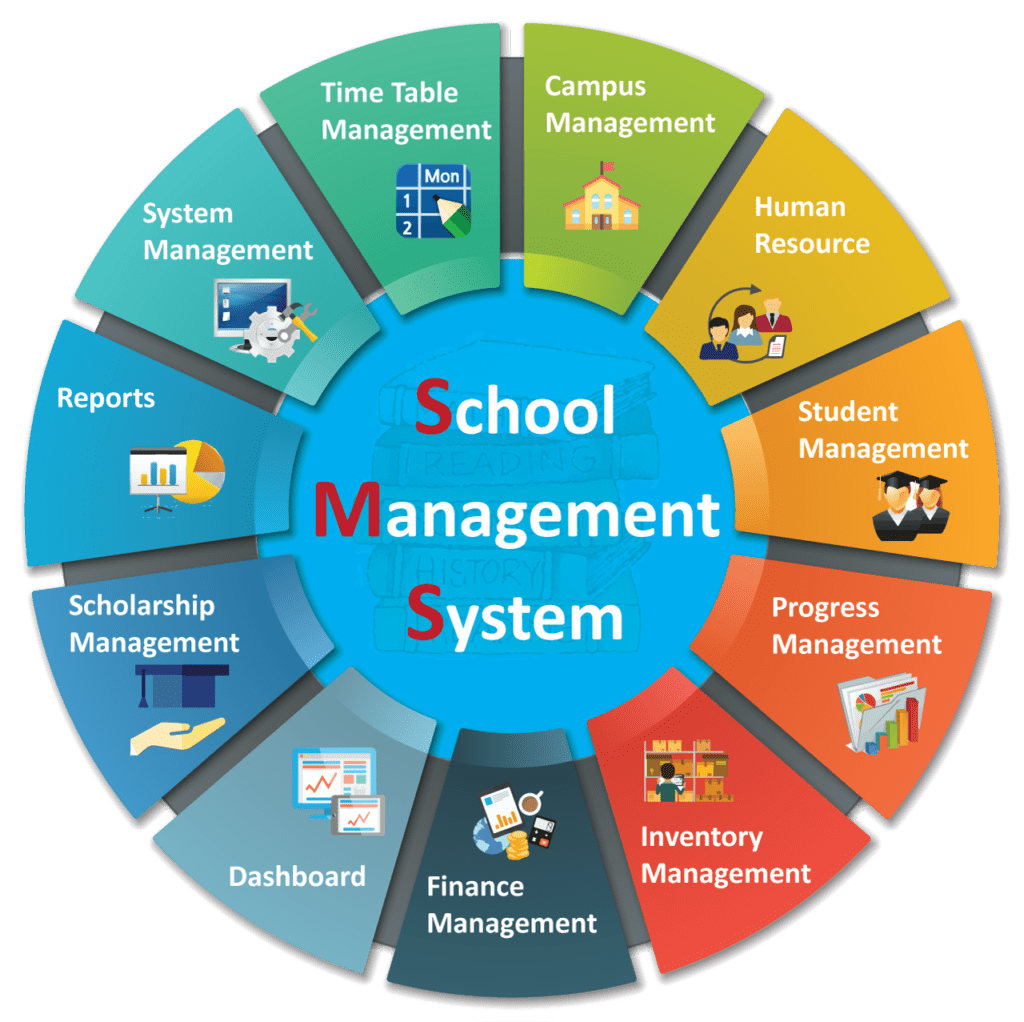
\includegraphics[scale=0.25]{Chapter1/sms}
\caption{School Management System}
\label{BMRDevice}
\end{center}
\end{figure}

SMS is a system that will provide you a bird�s eye view of the functioning of the entire educational institution. By using the latest technologies and help�s to make decision making a lot faster, effective and easier than ever before and will improve the overall quality of education of the institution.
The implementation of the system was done using PHP, html and SQL Server technologies, allowing system to be run in Windows OS. SMS managed education institution by simplifying and automating processes and addressing the needs of all stake holders helping them to be more efficient in their respective roles.
\section{Objectives}
The objective of this project describes how the aim of the project can be achieved. The
objectives of the projects are as follows:
\begin{itemize}
\item To choose appropriate methodology to follow for the development of School Management System.
\item To enhance the use and efficiency of authorized School management system.
\item To provide easy, safe, effective and attractive interface design that will be easy to
navigate.
\end{itemize}
\section{Project Scope}
Developments in information technology have been impacting upon educational organizations,
schools management have been using management system in order to improve the efficiency of
administrative. In management system, in order to ensure the efficiency and
effectiveness of school administration the design of right management system come to be key
issue. The system that the author is aiming to develop is a school management system that
will help to keep track of all data with better and reliability of a computerized system. The proposed school management system will come out with enhance functions and features which the current system does not possess, these functionalities will be explained in detail in the next coming chapter \cite{burke2003practice}.\\\\
The proposed system will control, manage data and process to support administrators, student, teachers, and secretaries. Other features that the proposed system will provide is proper security, which means the system, will be more secured that only the authorized personnel can access the
system. The system restricted that the student cannot access the system only the authorized users
can access the system. These features empower the administrators, teachers and secretary to spend less time managing administrative works and to avoid data redundancy and loss of data and other problems involve in the current system.
Information processing and sharing saves a significant amount of paper in the school. The new
features will add value to organization and improve the school�s image\cite{hedberg1992educational}.

\section{Features of Web-Based School Management System}
Following table will let us know about the different features of the web-based school management system.\\\\
\noindent With the rapid growth in the number and technology of instruments, the electric meter has played an increasingly important role in power systems. The power meter can be used to detect or measure the presence of voltage, current, and other parameters. The country has suffered from a power shortage for a decade, causing many disruptions to our domestic, industrial, and commercial activities. The is also one of the biggest problems of electricity theft by the private and industrial sector. It is necessary to explore different ways to solve the crisis and save the quantity of electricity supply and demand. One aspect of the problem is installing an efficient and correct accounting system, which is not possible unless we implement an intelligent and a pre-measurement system. In the current meter reading method, the digit manipulator determines the value or position of the needle with respect to the vision scale and causes the human reading to be compromised. In order to operate the larger
 instruments, the utility must read more Manpower meters. Especially with electricity meters, the most important thing is accuracy and regular reading many times higher than the test paid each month. Many
 meter readings not only tire the driver,
 accuracy cannot be guaranteed due to manual work. What is needed is a system that contains energy theft and allows customers to monitor energy use and be aware of the expected billing of
  energy consumed. This can be achieved through the use of a modern and intelligent
 meter reading system.\\\\\\\\
\\To obtain an acceptable detection accuracy for
 different types of electric meters, this report
 proposes a
 method of digital detection based on deep learning, which can be applied to different types and models of electric meters. There are two types of solutions for processes based on image recognition technology. The first category is OpenCV image recognition technologies. These
 methods were able to identify some objects such as numbers,
 image object outlines, etc., and can perform
 simple practical tasks in image processing. The first DNN-based
  technologies called segmentation-based methods, which always
 consist of two steps:
 segmentation and character recognition, B. Bissacco et al. first use a bounding box at position
 of the number in the image and then use a convolutional neural network (CNN)
 as the detection target. Newer methods based on DNN
  are known as non-segmentation methods, which use a recurrent neural network (RNN) to recognize the number in an image without fixing the position of objects\\\\\\
\\The design scheme uses an FPGA that combines the
 wireless transmission module. The FPGA chip is used to build a 32nd number
-bit Nios II soft-core processor, which replaces the traditional
 MCU structure, which takes advantage of the online configuration. ,
 expansion, and improved system performance offerings. Also, it can shorten the secondary development time. The
  nRF module is used to achieve\\\\\\\\
 wireless data transmission, which has the advantages of low cost, high
 transmission speed, and good communication quality. Practice
 shows that it can accurately complete data collection from
 meters and is also a trend in the development of the wireless
  meter reading system\\\\\\\\\\\\\\
\\PHS (Persona1 Handphone System), which enables wireless communication at a speed of 32 khps, is the original
 cell phone system in Japan. PHS uses a frequency band of approximately 1.9 GHz, which is higher than conventional digital cellular phone systems. PHS
 uses the "Micro Cell zone System" to make optimal use of the limited bandwidth. This system consists of relatively simple Cell-Station
 units, PHS designed it with the premise that it will be used in urban areas. This system is also used to find the location of a caller
. In addition, there are two modes in a PHS
 communication mode. One is the\\\\\\\\
 public communication mode (which incurs the required communication charges) that connects to a public network like a traditional
 cell phone, and the other is the transceiver mode (which incurs no
 connection charges) that can communicate between some
 terminals as a transceiver terminal without connecting it to the
 public network.
 Tool that automatically displays the value of pressure, temperature,
 and volume of gas consumption with a variety of
 sensors. This data is temporarily logged by a microcontroller
. The microcontroller connected to
 then sends the GSM / GPRS module as data from the communication device
  to the database server. The data is then processed in database
 and used as a customer invoice\\\\\\
\\In this article, a new chargeable electronic
 energy metering method is introduced, which
 automatically records the energy consumed, records this
 continuously and then sends\\\\\\\\ it to the billing center via the existing
  GPRS network. Finally, after processing, the collected
 data invoice is created with web-based system software and sent as SMS (
 short messaging system) to
 customer can monitor and analyze
 invoice generated every month from any Place of the world\\\\
\\In order to obtain acceptable detection accuracy for
 different types of electric meters, this article
 proposes a
 digital detection method based on deep learning, which can be applied to different types and models of
 electric meters\\\\\\
\\The designed system reduces the effort required to manually register
  energy meters. Furthermore, the data received at
 from the service provider side can be easily manipulated for the generation of invoices
  and other similar tasks. With this system we can
 record the measured values and control the delivery to the user.
 By adding software on the service provider side, the
 customer can be informed of the current meter reading, the current
 cycle bill, the line status and other parameters for the
 customer either by message, call telephone or Internet-based system\\\\\\
 \\Since most of the
 electricity meters are installed within the customer's residential buildings, the conventional approach to reading
  data is to enter private areas and read the meters. This approach faces problems such as:
 Door-to-door \\\\\\\\ data collection and involves
 inconvenience for customers. Applying AMR using the
 RF module can troubleshoot and improve
 power service performance, as well as increase customer satisfaction.In the next sections this paper will provide you better understanding of the proposal as well as its other technical and other details\\\\\\
 \\In order to obtain acceptable detection accuracy for
 different types of electric meters, this article
 proposes a
 digital detection method based on deep learning, which can be applied to different types and models of
 electric meters\\\\\\
\\The designed system reduces the effort required to manually register
  energy meters. Furthermore, the data received at
 from the service provider side can be easily manipulated for the generation of invoices
  and other similar tasks. With this system we can
 record the measured values and control the delivery to the user.
 By adding software on the service provider side, the
 customer can be informed of the current meter reading, the current
 cycle bill, the line status and other parameters for the
 customer either by message, call telephone or Internet-based system\\\\\\
 \\Since most of the
 electricity meters are installed within the customer's residential buildings, the conventional approach to reading
  data is to enter private areas and read the meters. This approach faces problems such as:
 Door-to-door \\\\\\\\ data collection and involves
 inconvenience for customers. Applying AMR using the
 RF module can troubleshoot and improve
 power service performance, as well as increase customer satisfaction.In the next sections this paper will provide you better understanding of the proposal as well as its other technical and other details.
 \section{Report Breakdown}
In this introduction chapter we have given an overview about the project, objectives of our projects, features which are the part of our project. In the chapter number two, we will provide a details about the tools/platform, hardware and software requirement specifications, in third chapter, We will describe how the database of the project is being implemented, in fourth chapter we will briefly discuss how the user interface of the project is being designed, and fifth chapter will contain the results, conclusions and future directions.
